\appendix
\chapter{Anhang}
\begin{table}[H]
    \caption{Spannungswerte bei der Konditionierung}
    \label{tab:Konditionierung}
    \begin{tabular}{lccc}
        \toprule
        Spannungsdifferenz [V] & Strom [mA] &	Widerstand [M$\Omega$] & Zeitinterval [min]\\   
        \midrule
            880  & 0,018 & 48,9 & 05:57\\
            980  & 0,021 & 46,7 & 06:39\\
            1080 & 0,024 & 45,0 & 05:36\\
            1200 & 0,028 & 42,9 & 07:26\\
            1330 & 0,032 & 41,6 & 07:20\\
            1450 & 0,036 & 40,3 & 04:13\\
            1580 & 0,040 & 39,5 & 04:41\\
            1700 & 0,044 & 38,6 & 04:43\\
            1825 & 0,048 & 38,0 & 06:01\\
            1940 & 0,052 & 37,3 & 05:10\\
            2060 & 0,056 & 36,8 & 07:45\\
            2160 & 0,059 & 36,6 & 05:57\\
            2270 & 0,063 & 36,0 & 05:59\\
            2380 & 0,068 & 35,0 & 06:16\\
            2480 & 0,071 & 34,9 & 06:27\\
            2600 & 0,071 & 36,6 & 06:02\\
            2700 & 0,080 & 33,8 & 06:46\\   
        \bottomrule     
    \end{tabular}
\end{table}

\begin{figure}
    \centering
    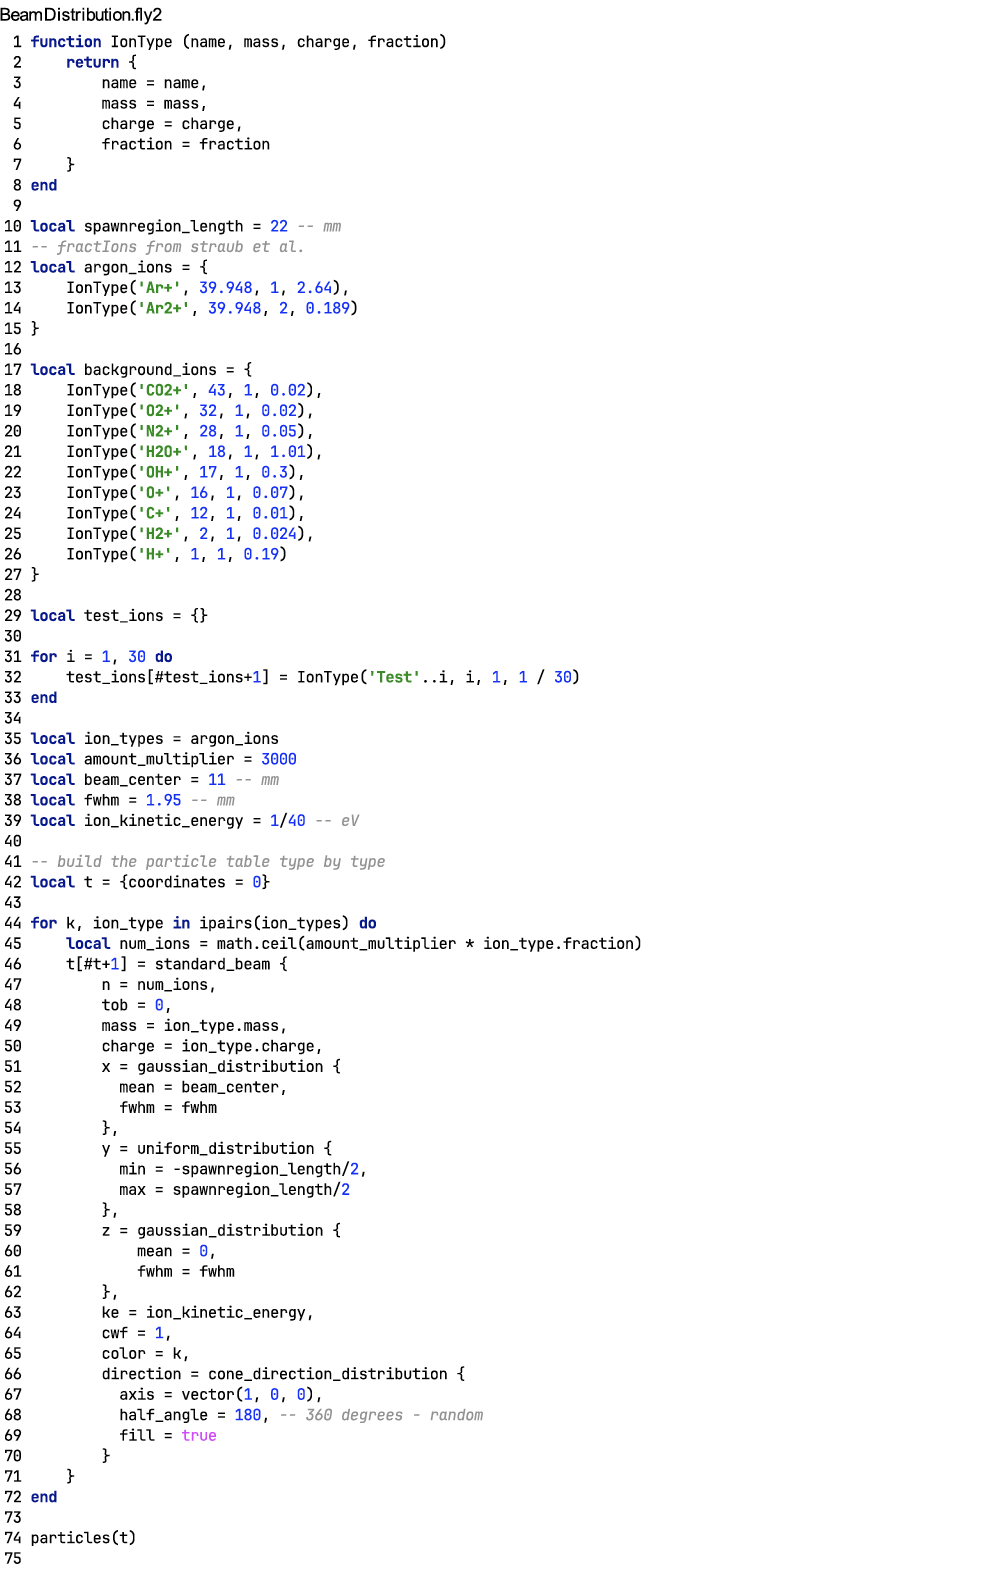
\includegraphics[width=1.05\textwidth]{Fly2.png}
    \caption[Ionenverteilung .fly2-File]{.fly2-File zur Definition der Ionenverteilung in \textit{SIMION} in der Programmiersprache Lua.}
    \label{fly2}
\end{figure}